\chapter{Kinematics}\label{chap:kinematics}
From the previous chapter we know the robot can be represented as a kinematic chain of rigid bodies and connected by revolute joints\cite{Siciliano}. The kinematics of the manipulator is described without consideration of the forces and torques causing its motion. This means that the description is geometric\cite{spong}. In this chapter the forward kinematics for this robotic manipulator is calculated and a method for solving the inverse kinematics is proposed. 

\section{Forward Kinematics}
The forward kinematics states the relationship between the end effector and the individual joints given the joint angles. The motion of the manipulator is obtained by composition of the elementary motions of each link with respect to the previous one\cite{Siciliano}. An easy way to get the forward kinematics is to use the Denavit-Hartenberg(DH) convention. Each homogeneous transformation $A_i$ is represented as a product of four basic transformations\cite{spong}: 
\begin{align}\label{eq:Ai}
A_i = \text{Rot}_{z,\theta_i}\text{Trans}_{z,d_i}\text{Trans}_{x,a_i}\text{Rot}_{x,\alpha_i}=
    \begin{bmatrix}
        c_{\theta_i} & -s_{\theta_i}c_{\alpha_i} & s_{\theta_i}s_{\alpha_i} & a_ic_{\theta_i}\\
        s_{\theta_i} & c_{\theta_i}c_{\alpha_i} & -c_{\theta_i}s_{\alpha_i} & a_is_{\theta_i}\\
        0 & s_{\alpha_i} & c_{\alpha_i} &d_i\\
        0 & 0 & 0 & 1
    \end{bmatrix}    
\end{align}
where $c_{\theta_i} = \cos{(\theta_i)}$ and $s_{\theta_i} = \sin{(\theta_i)}$, and the same for $\alpha$. $A_i$ is a transformation matrix which states the transformation between link number $i$ and link number $i-1$. This means that it is possible to get the transformation from the robot base to the end effector by multiplying each transformation matrix:
\begin{align*}
    T^i_j = A_{i+1}A_{i+2}...A_j, \quad i<j
\end{align*}
 $T^i_j$ states the transformation between each link and it has the form
 \begin{align*}
      T^i_j = 
      \begin{bmatrix}
          R^i_j & o^i_j\\
          0&1
      \end{bmatrix}, \quad i<j
 \end{align*}
 where $R^i_j = R^i_{i+1}R...R^{j-1}_j$ which is the orientation of $o_jx_jy_jz_j$ relative to $o_ix_iy_iz_i$. $o^i_j$ is the coordinate vector given in the world frame, which can be written as $o^i_j = o^i_{j-1}+R^{i}_{j-1}o^{j-1}_j$. This is useful when finding the Jacobian of the robot and to verify that the end effector is at the wanted position and has the wanted orientation in the Cartesian world frame. When finding the DH-parameters they have to satisfy the two following properties \cite{spong}
 \begin{itemize}
     \item The axis $x_n$ is perpendicular to the axis $z_{n-1}$
     \item The axis $x_n$ intersects the axis $z_{n-1}$
 \end{itemize}
In \figref{fig:dhf} the different axis are set with respect to the DH properties stated above\cite{Kinematics}.
\begin{figure}[htbp]
  \centering
  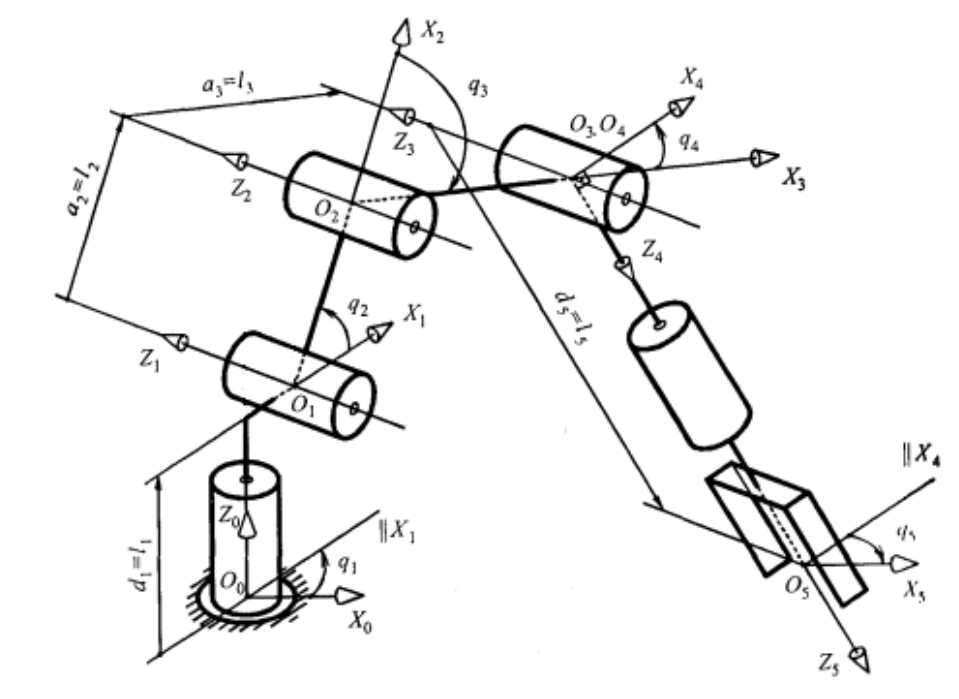
\includegraphics[width=.9\textwidth]{img/DHconv.png}
  \caption{Kinematic scheme of the manipulator\cite{Kinematics}}
  \label{fig:dhf}
\end{figure}\clearpage
\figref{fig:dhf}is used and the following DH parameters are found:
\begin{table}[htbp]
    \centering
    \caption{DH-parameters of the manipulator}
    \label{table:dhparms}
    \begin{tabular}{l c c c r}
         \toprule
         Link & $a_i$ & $\alpha_i$ & $d_i$ & $\theta_i$ \\
         \midrule
         1 & 0 & $-\frac{\pi}{2}$ & $d_1$ & $q_1$ \\
         2 & $a_2$ & 0 & 0 & $q_2$ \\ 
         3 & $a_3$ & 0 & 0 & $q_3$\\
         4 & 0 & $\frac{\pi}{2}$ & 0 & $q_4$\\
         5 & 0 & 0 & $d_5$ & $q_5$\\
         \bottomrule
    \end{tabular}
\end{table}\\
where $d_1 = 0.0506m$, $a_2 = 0.1347m$, $a_3 = 0.0712m$ and $d_5 = 0.1765m$ for the model. As previously mentioned in Section \ref{sec:massInert}, the real values need to be measured properly since the data sheet of the robot is insufficient and this is just guesstimated values\cite{Crustcrawler}. 
Now it is possible to calculate $A_i$ from \eqref{eq:Ai} for each link: 
\begin{align*}
A_1 &= \begin{bmatrix} 
            c_1 & 0 & -s_1 & 0\\
            s_1 & 0 & c_1 & 0\\
            0 & -1 & 0 & d_1\\
            0 & 0 & 0 & 1
        \end{bmatrix},
A_2 = \begin{bmatrix} 
            c_2 & -s_2 & 0 & a_2c_2\\
            s_2 & c_2 & 0 & a_2s_2\\
            0 & 0 & 1 & 0\\
            0 & 0 & 0 & 1
        \end{bmatrix},
A_3 = \begin{bmatrix} 
            c_3 & -s_3 & 0 & a_3c_3\\
            s_3 & c_3 & 0 & a_3s_3\\
            0 & 0 & 1 & 0\\
            0 & 0 & 0 & 1
        \end{bmatrix}\\
A_4 &= \begin{bmatrix} 
            c_4 & 0 & s_4 & 0\\
            s_4 & 0 & -s_4 & 0\\
            0 & 1 & 0 & 0\\
            0 & 0 & 0 & 1
        \end{bmatrix},
A_5 = \begin{bmatrix} 
            c_5 & -s_5 & 0 & 0\\
            s_5 & c_5 & 0 & 0\\
            0 & 0 & 1 & d_5 \\
            0 & 0 & 0 & 1
        \end{bmatrix}
\end{align*}
 and then calculate $T_i^0$:
\begin{subequations}
    \begin{align}
        T_1^0 &= A_1 =
        \begin{bmatrix}\label{eq:T1}
            c_1 & 0 & -s_1 & 0\\
            s_1 & 0 & c_1 & 0\\
            0 & -1 & 0 & d_1\\
            0 & 0 & 0 & 1
        \end{bmatrix}
    \end{align}
    \begin{align}
        T_2^0 &= A_1A_2 =
        \begin{bmatrix}\label{eq:T2}
            c_1c_2 & -c_1s_2 & -s_1 & a_2c_1c_2\\
            s_1c_2 & -s_1s_2 & c_1 & a_2s_1c_2\\
            -s_2 & -c_2 & 0 & d_1 - a_2s_2\\
            0 & 0 & 0 & 1
        \end{bmatrix}
        \end{align}
        \begin{align}
        T_3^0 &= A_1A_2A_3=
        \begin{bmatrix}\label{eq:T3}
            c_{23}c_1 & -c_1s_{23} & -s_1 & c_1(a_3c_{23} + a_2c_2)\\
            c_{23}s_1 & -s_1s_{23} & c_1 & s_1(a_3c_{23} + a_2c_2)\\
            -s_{23} & -c_{23} & 0 & d_1 - a_3s_{23}-a_2s_2\\
            0 & 0 & 0 & 1
        \end{bmatrix}
        \end{align}
        \begin{align}        
        T_4^0 &= A_1A_2A_3A_4=
        \begin{bmatrix}\label{eq:T4}
            c_1c_{234} & -s_1 & c_1s_{234} & c_1(a_3c_{23} + a_2c_2)\\
            s_1c_{234} & c_1 & s_1s_{234} & s_1(a_3c_{23} + a_2c_2)\\
            -s_{234} & 0 & c_{234} & d_1 - a_3s_{23} - a_2s_2\\
            0 & 0 & 0 & 1
        \end{bmatrix}
        \end{align}
        \begin{align}        
        \begin{split}
            T_5^0 &= A_1A_2A_3A_4A_5\\ &=
            \begin{bmatrix}\label{eq:T5}
                c_1c_{234}c_5 - s_1s5 & -s_1c_5 - c_1c_{234}s_5 & c_1s_{234} & c_1(a_3c_{23} + a_2c_2 + d_5s_{234})\\
                s_1c_{234}c_5 + c_1s_5 & c_1c_5 - s_1c_{234}s_5 & s_1s_{234} & s_1(a_3c_{23} + a_2c_2 + d_5s_{234})\\
                -s_{234}c_5 & s_{234}s_5 & c_{234} & d_1 - a_3s_{23} - a_2s_2 + d_5c_{234}\\
                0 & 0 & 0 & 1
            \end{bmatrix}
        \end{split}
     \end{align}
\end{subequations}
where $s_{ijk} = \sin{(q_i + q_j + q_k)}$ and the same for $c_{ijk}$. Notice that the zero configuration, i.e. all joint angles are zero, is not the configuration as pictured in \figref{fig:RG} where the manipulator is standing straight up which is the zero position when spawning the model with URDF. This can either be handled in the URDF by changing the zero configuration or by subtracting the difference from $q_i$.
%The $T_i^0$ matrix can be sectioned into
%\begin{align*}
 %T_i^0 = 
  %  \begin{bmatrix}
   %     \bm{R}(\bm{q}) & \bm{p}(\bm{q})\\
    %    \bm{0}^T & 1
    %\end{bmatrix}    
%\end{align*}

%-----------------------------------------------------------------------------------------
\begin{comment}
\begin{align*}
    T^0_5 &= A_1A_2A_3A_4A_5\\
    &= 
    \begin{bmatrix}
        c_1c_{234}c_5 + s_1s_5 & -c_1c_{234}s_5+s_1c_5 & -c_1s_{234} & c_1(-d_5s_{234} + a_3c_{23} + a_2c_2)\\
        c_1c_{234}c_5 - s_1s_5 & -s_1c_{234}s_5-c_1c_5 & -s_1s_{234} & s_1(-d_5s_{234} + a_3c_{23} + a_2c_2) \\
        -s_{234}c_5 & s_{234}s_5 & -c_{234} &d_1 - a_2s_2 - a_3s_{23} - d_5c_{234}\\
        0 & 0 & 0 & 1\\
    \end{bmatrix}\\
    &=
    \begin{bmatrix}
        \bm{R}(\bm{q}) & \bm{p}(\bm{q})\\
        \bm{0}^T & 1
    \end{bmatrix}
\end{align*}
\end{comment}
%-----------------------------------------------------------------------------------------

%\subsection{Reduced form }
%In \eqref{eq:T5} the orientation and position is described with a position vector and a rotation matrix. The rotation matrix can some times be a bit abstract and it can be hard to see what the orientation actually is. Along with simplifying some calculation and coding it can therefore be useful to represent the orientation as Euler Angles \cite{Siciliano}. The Euler angles that we choose is the \textit{Roll-Pitch-Yaw angles(RPY)} or ZYX angles. This means that we can decompose the orientation of the end-effector into three rotations, $\phi = [\varphi,\vartheta,\psi]^T$ where
%\begin{align*}
%    \varphi &= \atantwo{(r_{21},r_)}
%\end{align*}




\subsection{Jacobian Matrix}
The geometric Jacobian gives the relationship between the joint velocities and the linear and angular velocities of the end effector\cite{Siciliano,spong}. As we already know the forward kinematics can be written as:
\begin{align*}
    T(q) = 
    \begin{bmatrix}
        R(q) & p(q)\\
        0 & 1
    \end{bmatrix}
\end{align*}
we want to express the linear velocity $\dot{p}$ and angular velocity $\omega$ as a function of the joint velocities $\dot{q}$. In \cite{Siciliano} the relations is stated as:
\begin{equation}
    \begin{aligned}\label{eq:velo}
        \dot{p} &= J_P(q)\dot{q}\\
        \omega&= J_O(q)\dot{q}
    \end{aligned}
\end{equation}
where $J_O$ with dimensions (3 $\times$ n) is the relation between the joint velocities $\dot{q}$ and the end-effector linear velocity $\dot{p}$, and the (3 $\times$ n) matrix $J_O$ is the relation between the joint velocities $\dot{q}$ and the end-effector angular velocity $\omega$. Equation \eqref{eq:velo} can be written as
\begin{align*}
    v_e = 
    \begin{bmatrix}
        \dot{p} \\ \omega
    \end{bmatrix}
    = J(q)\dot{q}
\end{align*}
where
\begin{align*}
    J = 
    \begin{bmatrix}
        J_P \\ J_O
    \end{bmatrix}
\end{align*}
which is the geometric Jacobian matrix. The elements of 
$$
J = 
\begin{bmatrix}
    j_{P1} & & j_{Pn}\\
    &...&\\
    j_{O1} & & j_{On}
\end{bmatrix}
$$
can be calculated in the following way:
\begin{align*}
    \begin{bmatrix}
        j_{Pi}\\j_{Oi}
    \end{bmatrix}
    =
    \begin{cases}
        \begin{bmatrix} z_{i-1}\\ 0 \end{bmatrix} & \text{for a prismatic joint}\\
        \begin{bmatrix} z_{i-1} \times (p_e-p_{i-1}) \\ z_{i-1} \end{bmatrix} & \text{for a revolute joint}
    \end{cases}
\end{align*}
Since our manipulator only has revolute joints, the geometric Jacobian becomes
\begin{align*}
    J(q) = 
    \begin{bmatrix}
        z_0 \times (p_5-p_0) & 
        z_1 \times (p_5-p_1) & 
        z_2 \times (p_5-p_2) & 
        z_3 \times (p_5-p_3) & 
        z_4 \times (p_5-p_4) \\
        z_0 &
        z_1 &
        z_2 &
        z_3 &
        z_4
    \end{bmatrix}
\end{align*}
From when the forward kinematics were calculated each position vector $p_i$ can be directly obtained from the equations \eqref{eq:T1} - \eqref{eq:T5}:
\begin{align*}
    p_0 = \begin{bmatrix} 0 \\ 0 \\ 0 \end{bmatrix}    \quad
    p_1 = \begin{bmatrix} 0 \\ 0 \\ d_1\end{bmatrix}    \quad
    p_2 = \begin{bmatrix} a_2c_1c_2\\ a_2s_1c_2\\ d_1 - a_2s_2\end{bmatrix}   \quad 
    p_3 = \begin{bmatrix} c_1(a_3c_{23} + a_2c_2) \\ s_1(a_3c_{23} + a_2c_2) \\ d_1 - a_3s_{23}-a_2s_2 \end{bmatrix}  \\  
    p_4 = \begin{bmatrix} c_1(a_3c_{23} + a_2c_2) \\ s_1(a_3c_{23} + a_2c_2) \\ d_1 - a_3s_{23}-a_2s_2\end{bmatrix}  \quad  
    p_5 = \begin{bmatrix} c_1(a_3c_{23} + a_2c_2 + d_5s_{234}) \\ s_1(a_3c_{23} + a_2c_2 + d_5s_{234}) \\ d_1 - a_3s_{23} - a_2s_2 + d_5c_{234} \end{bmatrix}    
\end{align*}
The next step is to find $z_{i-1}$. Reference \cite{Siciliano} states that $z_{i-1}$ is given by the third column of the rotation matrix $R_{i-1}^0$. $R_{i-1}^0$ is already given in $T_i^0$, By looking at \eqref{eq:T1} - \eqref{eq:T5} the following values of $z_{i-1}$ is given:
\begin{align*}
    z_0 &= \begin{bmatrix}0\\0\\1\end{bmatrix},
    z_1 = \begin{bmatrix}-s_1\\c_1\\0\end{bmatrix},
    z_2 = \begin{bmatrix}-s_1\\c_1\\0\end{bmatrix},
    z_3 = \begin{bmatrix}-s_1\\c_1\\0\end{bmatrix},
    z_4 = \begin{bmatrix}c_1s_{234}\\s_1s_{234}\\c_{234}\end{bmatrix}
\end{align*}
now we got everything needed to compute the geometric Jacobian and the result is presented below.
\begin{align*}
    J(q) &= \\
    &\begin{bmatrix}
        -s_1(a_3c_{23} + a_2c_{2} + d_5s_{234}) & 
        -c_1(a_3s_{23} + a_2s_{2} - d_5c_{234}) & 
        -c_1(a_3s_{23} - d_5c_{234})            & 
        c_1d_5c_{234}                           & 
        0\\
        c_1(a_3c_{23} + a_2c_{2} + d_5s_{234})  & 
        -s_1(a_3s_{23} + a_2s_{2} - d_5c_{234}) & 
        -s_1(a_3s_{23} - d_5c_{234})            & 
        s_1d_5c_{234}                           & 
        0\\
        0                                       &
        -a_3c_{23}- a_2c_2 - d_5s_{234}         &
        -a_3c_{23} - d_5s_{234}                 &
        -d_5s_{234}                             &
        0\\
        0                                       &
        -s_1                                    &
        -s_1                                    &
        -s_1                                    &
        c_1s_{234}\\
        0                                       &
        c_1&
        c_1&
        c_1&
        s_1s_{234}\\
        1& 0 & 0 & 0 & c_{234}
    \end{bmatrix}
\end{align*}
which has the full rank of $5$. 

















\section{Inverse Kinematics}
The forward kinematics establishes the relationship between the joint variables and the position and orientation of the end effector. The problem of inverse kinematics is to find the joint variables when the position and orientation of the end effector is given. This is wanted because the desired position or path is given in Cartesian coordinates. Unfortunately the inverse kinematics problem is not as easy and straight forward as the forward kinematics problem. Reference \cite{Siciliano} lists up several reasons the inverse kinematics problem is more complex:
\begin{itemize}
    \item The equations to solve are in general nonlinear, and thus it is not always possible to find a closed-form solution.
    \item Multiple solutions may exist.
    \item Infinite solutions may exist, e.g., in the case of a kinematically redundant manipulator.
    \item There might be no admissible solutions, in view of the manipulator kinematic structure.
\end{itemize}
There are different methods of solving the inverse kinematics problem. One method is to compute an algebraic solution. The desired solution is a function with orientation and position of the end effector as input, and the output is the joint angles needed to satisfy the input. In our case where we have a 5 DOF robot arm the equations becomes too large and too difficult to solve\cite{spong}. By looking at the equation $T_5^0=H$ where $T_5^0$ is given in \eqref{eq:T5} and $H$ is the desired transformation matrix of the end effector. It shows us that it gives a complex set of equations to solve. Another thing that must be considered is that not all joints in our system can rotate 360 degrees either so if a solution is to be found it may not work because of the limitations of the robot manipulator. \\\\
It is also possible to use a geometric approach where the thought is to find the joint angels by projecting the manipulator onto the previous plane, and solve it using trigonometry\cite{spong}. Both \cite{Siciliano} and \cite{spong} uses simple manipulators and special cases where simplifications can be made, and do not cover our 5 DOF manipulator.\\\\
After some research in making a inverse kinematics solver from the bottom and up, it was found that this will not yield satisfactory results since existing and better solutions is already made. The choice was therefore to use an already existing solver. Several solvers were considered but the most commonly used did not have good support for a 5 DOF robot manipulator\cite{Ikfast,kdl}, but after some research the choice fell upon a MATLAB robotics toolbox\cite{MatlabRobTool}. The toolbox has a great interface with ROS which makes it easy to get and send messages via subscribers and publishers\cite{MatlabRobTool,ROSWiki}. A useful part is that it is possible to include the URDF file where MATLAB creates a robot object and represent the robot manipulator as a rigid body tree. In other words it is just the way MATLAB parses the URDF file. In \figref{fig:showRovs} the MATLAB function $show(robot)$ is used and one can see the visualization of the robot. This can be used to check solutions of inverse kinematics and path planning and it can be thought as a simpler version of rviz.  \\\\
\begin{figure}[htbp]
  \centering
  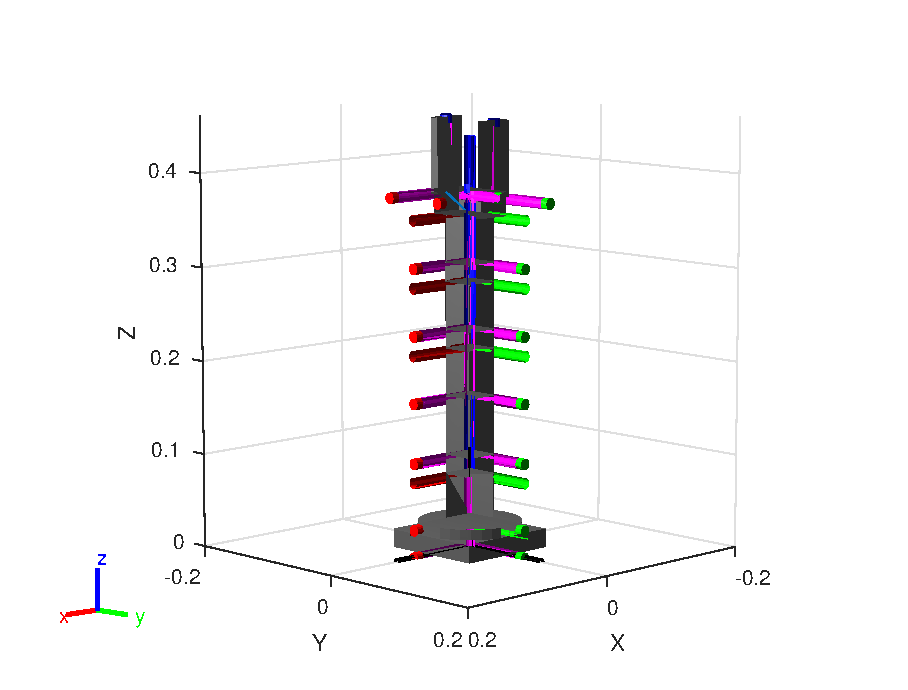
\includegraphics[width=.9\textwidth]{img/showRobs.eps}
  \caption{MATLAB visualization of the robot using URDF}
  \label{fig:showRovs}
\end{figure}
In \lstref{lst:robotinit} seen below, the URDF file of the robot is imported into the workspace of MATLAB. Then the inverse kinematics solver object is also created. The initial solver of the inverse kinematics problem is the \textit{Broyden–Fletcher–Goldfarb–Shanno} (BFGS) algorithm which is an iterative, gradient-based optimization method that starts with an initial guess to minimize a cost function \cite{MatlabRobTool}. The other solving algorithm is the \textit{Levenberg-Marquardt} algorithm, which is not as good if the initial point is far away from the solution, but it is faster if the intial point are close to the solution. So if the goal is to do path following, it could be a good choice to use \textit{Levenberg-Marquardt}\cite{MatlabRobTool}. 
\begin{lstlisting}[caption={MATLAB code of creating and specifying an inverse kinematics object},label={lst:robotinit},language=Matlab]
robot = importrobot('robot.urdf');
ik = robotics.GeneralizedInverseKinematics('RigidBodyTree',robot);
ik.ConstraintInputs={'joint','position','orientation'};
ik.SolverParameters.SolutionTolerance = 0.00001;
ik.SolverParameters.GradientTolerance = 0.000001;
ik.SolverParameters.MaxTime = 0.1;
ik.SolverParameters.AllowRandomRestart = 0;
\end{lstlisting}
The \lstref{lst:gik} shows an example of finding the inverse kinematics. Here we want the end effector to reach the position $p_d$ with the orientation $o_d$. It is also wanted to have some constraints such that the solution is at a feasible configuration which is seen at line 6 to 10. Again the datasheets does not state the operational limits of the joints 2,3 and 4, so the bounds has been guessed. The bounds of the twisting joints 1 and 5 are set to $\pm \pi$ to avoid solutions past these bounds e.g. rotate one and a half round is not necessary when it can rotate half a round. So it is just as security that the solver does not over complicate its solution. \\\\
\begin{lstlisting}[caption={MATLAB code for specifying $p_d$, $o_d$ and joint bounds which is used to find a solution of the inverse kinematics problem},label={lst:gik},language=Matlab]
posTgt = robotics.PositionTarget('end_effector');
posTgt.TargetPosition = pd';
orTgt = robotics.OrientationTarget('end_effector');
orTgt.TargetOrientation = eul2quat(od');
jointConst = robotics.JointPositionBounds(robot);
jointConst.Bounds = [-pi,pi;
                -3*pi/4,3*pi/4
                -3*pi/4,3*pi/4
                -3*pi/4,3*pi/4
                -pi,pi];
initialguess = robot.homeConfiguration;
[configSoln,solInfo] = ik(initialguess,jointConst,posTgt,orTgt);
qd = [configSoln(:).JointPosition]';
\end{lstlisting}
In \figref{fig:oath} a random path has been generated. It is inside the configuration space of the robot. The projection onto the xy-plane, xz-plane and yz-plane plane is also plotted for convenience to get a better feel of the 3D path. The next goal is to generate a circular motion such that it would start and end in the same point. Below in \lstref{lst:path} the process of generate this simple path is shown. The desired orientation in ZYX Euler angles is $o_d = [0,0,0]^T$ which in means that the desired orientation is up.
\begin{lstlisting}[caption={MATLAB code for creating path},label={lst:path},language=Matlab]
t = 0:steplength:2*pi+steplength
xpath = 0.035*cos(t)+0.09;
ypath = 0.035*sin(t)+0.09;
zpath = 0.050*sin(t)+0.25;
path = [xpath;ypath;zpath];
\end{lstlisting}
In \figref{fig:compa} the generated path from \lstref{lst:path} and the calculated path from the inverse kinematics is plotted. Equation \eqref{eq:T5} was used to convert the joint paths to xyz coordinates in the world frame. The results is good and the largest error is an error of $0.0092$ radians which corresponds to approximately $0.5$ degrees. The mean error is $8.54\cdot10^{-6}$ radians. 
\def\picsSiz{1.08}
\begin{figure*}[htbp]
    \centering
    \begin{subfigure}[htbp]{0.48\textwidth}
        \centering
        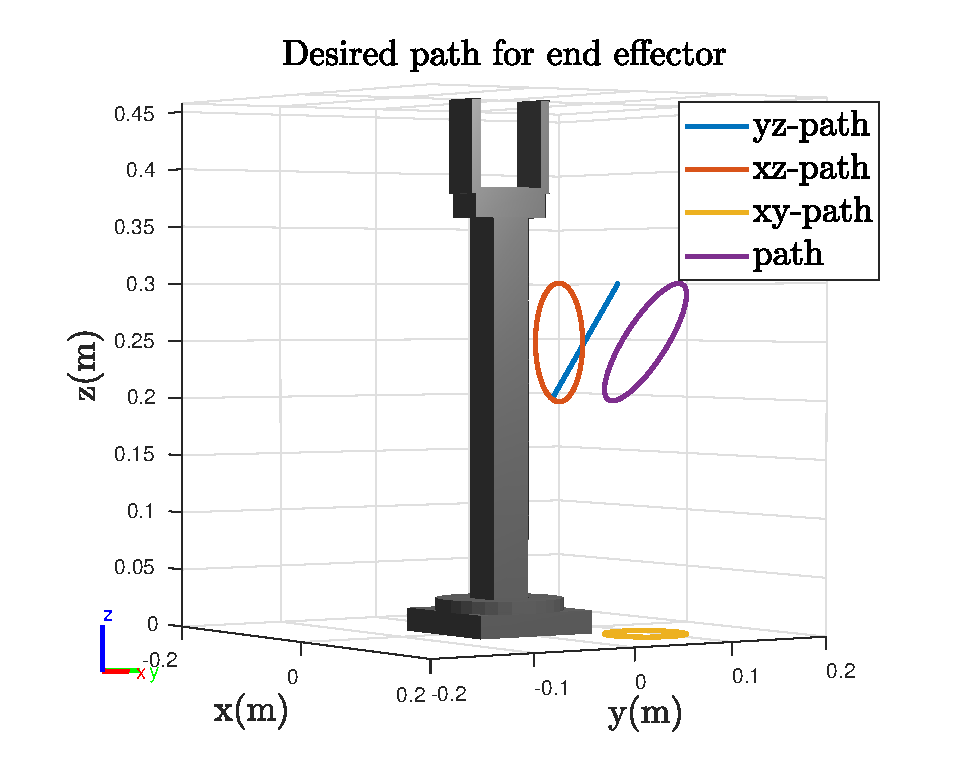
\includegraphics[width = \picsSiz\linewidth]{img/pathRob.eps}
        \caption{An arbitrary generated path for the end effector}
        \label{fig:oath}
    \end{subfigure}
    ~ 
    \begin{subfigure}[htbp]{0.48\textwidth}
        \centering
        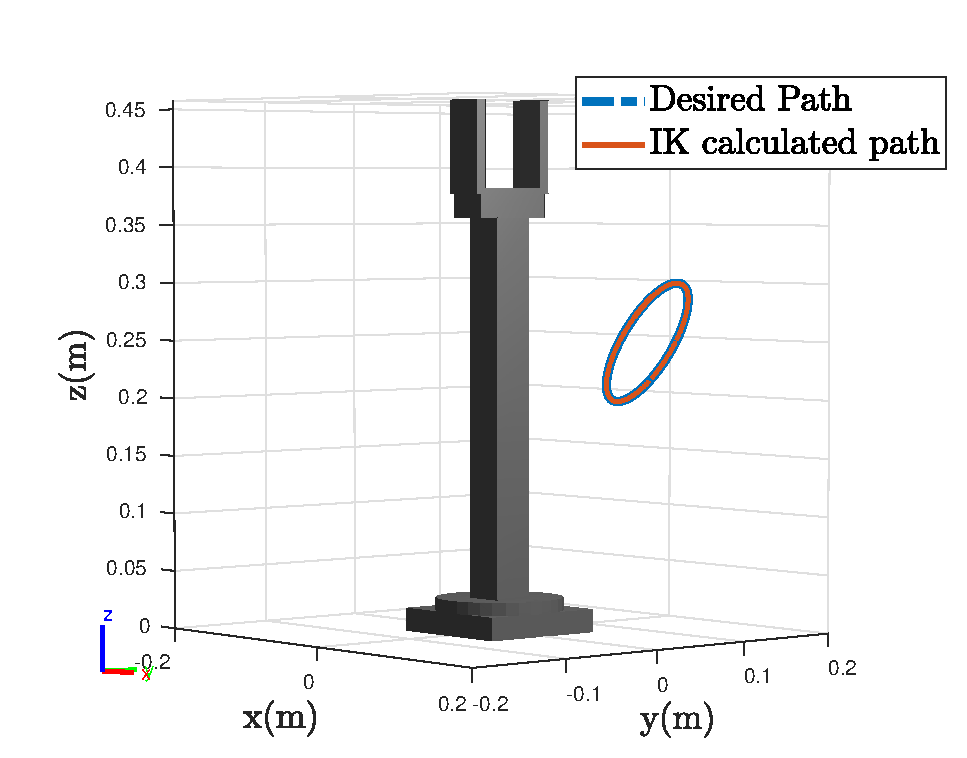
\includegraphics[width = \picsSiz\linewidth]{img/compIK.eps}
        \caption{Comparison by the ran}
        \label{fig:compa}
    \end{subfigure}
    \caption{Testing the inverse kinematic solver}
    \label{fig:IKcom}
\end{figure*}
In \figref{fig:outOC} some of the path is moved outside the configuration space of the robot and one can see that the solver makes the path at its best effort. In other words, if given a path, it will follow it until it goes out of the configuration space, and then it will follow the path that minimizes the cost function of the solver. 

\begin{figure}[htbp]
  \centering
  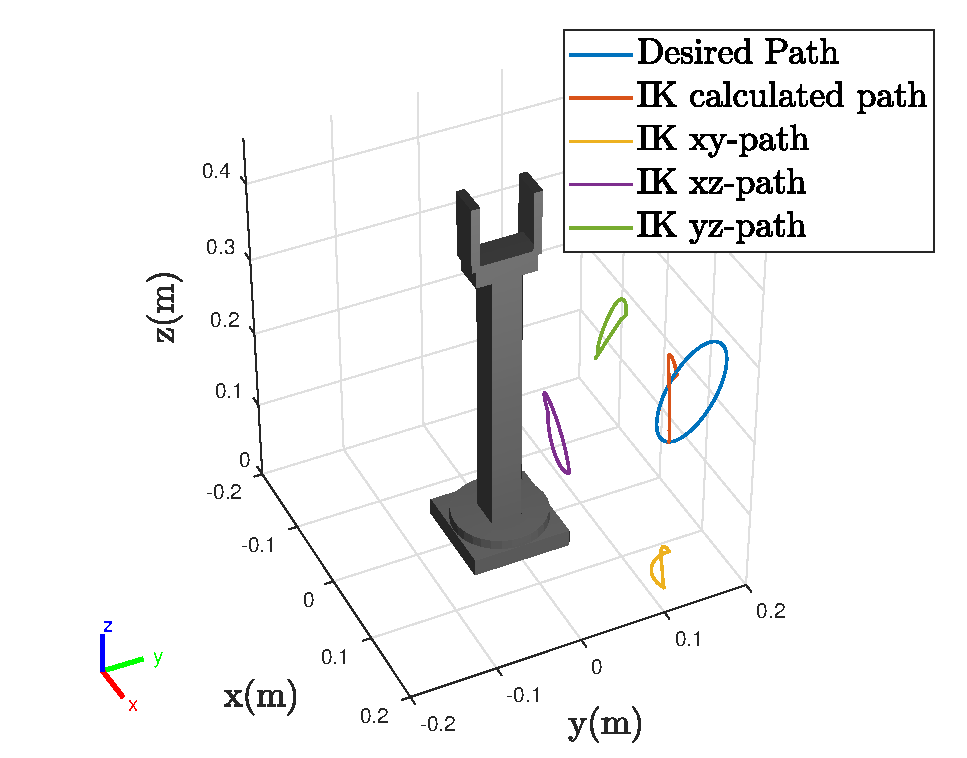
\includegraphics[width=.8\textwidth]{img/outOS.eps}
  \caption{Test of the solver when the path is partially out of the configuration space}
  \label{fig:outOC}
\end{figure}

In this chapter the forward kinematics has been found along the inverse kinematics. All these are important aspects of a robot system and will used in further work and in this project. 







































\begin{comment}


\cite{Siciliano} states that one can use the Jacobian of the system to calculate the inverse kinematics:

\begin{align}\label{eq:algo}
\dot{\bm{e}} = \dot{\bm{x}}_d - \bm{J}_A(\bm{q})\dot{\bm{q}}
\end{align}

In \figref{fig:inverseAlgo} the inverse kinematics algorithm is stated. From the figure one can see that 
$$
\dot{\bm{q}} = \bm{J}_A^{-1}(\bm{q})(\dot{\bm{x}}_d + \bm{K}e)
$$
where K is a positive definite diagonal matrix which makes the resulting system \eqref{eq:algo} into the linear system
\begin{align*}
    \dot{\bm{e}} + \bm{K}e = \bm{0}
\end{align*}


\begin{figure}[htbp]
  \centering
  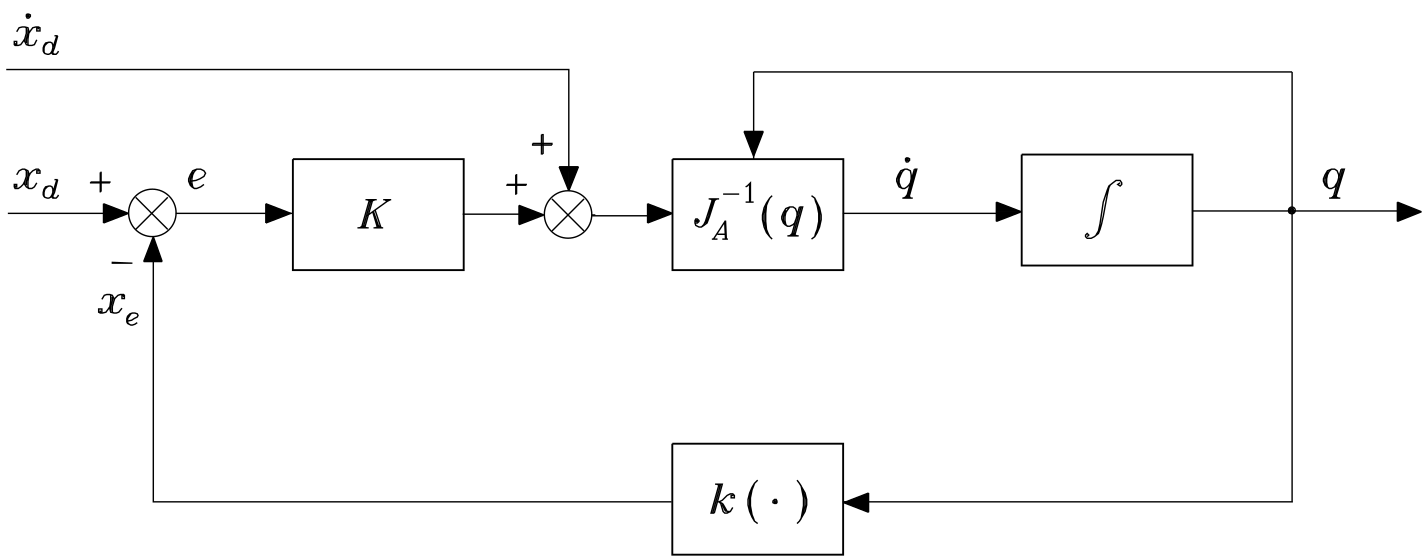
\includegraphics[width=.9\textwidth]{img/inverseKin.png}
  \caption{Inverse kinematics algotihm with Jacobian inverse. Source \cite{Siciliano}.}
  \label{fig:inverseAlgo}
\end{figure}

\subsubsection*{Analytical Jacobian}
To use the algorithm in \figref{fig:inverseAlgo} the analytical Jacobian is needed. In \cite{Siciliano} the following relationship is given
\begin{align*}
    \bm{J}_A =
    \begin{bmatrix}
        \bm{I} & \bm{0}\\ 0 & \bm{T}^{-1}(\bm{\phi_e})
    \end{bmatrix}
    \bm{J}(\bm{q})
\end{align*}

where $\bm{\phi_e} = [\phi,\theta,\psi]^T$ is the orientation of the end-effector frame relative to the base frame given by the Euler angles ZYZ. From \eqref{eq:T5} the rotation matrix from the base frame to end-effector is
\begin{align*}
    \bm{R}_5^0 &= 
    \begin{bmatrix}
        r_{11} & r_{12} & r_{13}\\
        r_{21} & r_{22} & r_{23}\\
        r_{31} & r_{32} & r_{33}
    \end{bmatrix}
    =
    \begin{bmatrix}
        c_1c_{234}c_5 - s_1s_5 & -s_1c_5 - c_1c_{234}s_5 & c_1s_{234}\\
        s_1c_{234}c_5 + c_1s_5 & c_1c_5 - s_1c_{234}s_5 & s_1s_{234}\\
        -s_{234}c_5 & s_{234}s_5 & c_{234} 
    \end{bmatrix}
\end{align*}

The ZYZ Euler angles are then


\begin{align*}
    \phi &= atan2(r_{21},r_{11}) = atan2(s_1c_{234}c_5 + c_1s_5,c_1c_{234}c_5 - s_1s_5)\\
    \theta &= atan2\left(-r_{31},-\sqrt{r_{32}^2+r_{33}^2}\right) = atan2\left(s_{234}c_5,-\sqrt{s_{234}s_5^2+c_{234}^2}\right)\\
    \psi &= atan2(r_{32},r_{33}) = atan2(s_{234}s_5,c_{234})
\end{align*}

The angular velocity $\bm{\omega}_e$ and $\bm{T}(\bm{\alpha})$ is given as

\begin{align*}
    \bm{\omega} = 
    \begin{bmatrix}
        0 & -s_\phi & c_\phi s_\theta\\
        0 & c_\phi & s_\phi s_\theta\\
        1 & 0 & c_\theta
    \end{bmatrix}
    \begin{bmatrix}
        \dot{\phi}\\\dot{\theta}\\\dot{\psi}
    \end{bmatrix}
    =
    \bm{T}(\bm{\phi}_e)\dot{\bm{\phi}}_e
\end{align*}
The determinant of $\bm{T}$ is $-s_\theta$ which means that one cannot invert for $\theta = 0,\pi$. This singularity is also the singularity of the geometric Jacobian. 








\section{Motion planning}




If the desired position is $p$ and the desired orientation is $R$. Then in \cite{Kinematics}, the inverse kinematics are given as: 

\begin{align*}
    q_1 &= \tan^{-1}{\left(\frac{p_y}{p_x}\right)}\\
    q_2 &= atan2\left( a(a_2+a_3c_3) - ba_3s_3, aa_3s_3 + b(a_2+a_3c_3) \right)\\%atan2
    q_3 &= \cos^{-1}{\left(\frac{a^2+b^2-a^2_2-a^2_3}{2a_2a_3}\right)}\\
    q_4 &= q_{234} - q_2 - q_3\\
    q_5 &= c_{234}q_1-2atan(R_{21},R_{11})
\end{align*}

where $a = d_1 - d_5c_{234}-p_z$, $b = p_xc_1 + p_ys_1+d_5s_{234}$ and $-\frac{\pi}{2}<q_1 < \frac{\pi}{2}$. $q_{234} = atan2\left(\frac{p_x}{c_1p_x+s_1p_y})\right)$


\end{comment}